\documentclass[english,titlepage]{article}

\usepackage[pdftex]{graphicx}
\usepackage[tmargin=0.8in, bmargin=0.8in, rmargin=0.8in, lmargin=0.8in]{geometry}
\usepackage{setspace}
\usepackage{booktabs}
\usepackage{bigstrut}
\usepackage{subfigure}
\usepackage{float}
\usepackage{hyperref}
\usepackage{longtable}
\usepackage{rotating}
\usepackage[inline]{enumitem}
\usepackage{xspace}
%\usepackage{fullpage}
\usepackage{svg}
\usepackage{amsmath}
\usepackage{comment}
\usepackage{amssymb}
\usepackage{amsfonts}
\usepackage{multicol}
\usepackage{listings}
\usepackage{float} % use for putting pics where you want. Replace the ht with H
\usepackage{verbatim}
\usepackage{placeins}
\usepackage{caption}
\usepackage[most]{tcolorbox}
\setlength{\parindent}{0cm} % removes paragraph indentation 

\makeatletter
\usepackage{fancyhdr}
\fancyhead{}
\fancyhead[L]{\bfseries Michael Mauboussin}
\fancyhead[C]{\bfseries Expectations Investing}
\fancyhead[R]{\bfseries Columbia Business School}
\fancyfoot[C]{\thepage}
\fancyfoot[L]{Rishi Ratan}
\fancyfoot[R]{Jan 2022}
\pagestyle{fancy}
\renewcommand{\headrulewidth}{0.5pt}
\renewcommand{\footrulewidth}{0.5pt}
\makeatother
\usepackage{babel}
\begin{document}
\title{\textbf{Expectations Investing} \\ 
\date{}
\doublespacing{Key Learnings Summary}}
\maketitle
\section{Key Shifts in the market since 2001}
\begin{itemize}
    \item \textbf{Shift from \emph{active to passive} investing}: Index funds and ETFs are the prominent investment asset classes rather than stock picking. 
    \item \textbf{Rise of intangible investments}: Companies today invest substantially more in intangible assets because they appear on the income statement as an expense, while tangible investments are recorded as assets on the balance sheet. 
    \item \textbf{Shift from Public to Private Equity}: There are ~1/3 fewer public companies listed in the US today compared to 2001. VC an PE have become the new preferred asset classes for investors and operators are staying private longer to avoid scrutiny endured in the public markets. 
    \item \textbf{Changes in Accounting Rules}: In the 1990s, stock-based compensation (SBC) consisted primarily of employee stock options (ESOPs) that were \emph{not} expensed on the income statement. 
                                                Today, SBC is primarily in the form of restricted stock units (RSUs) that are expensed on the income statement. 
                                                Therefore, both the form of renumeration and how it is accounted for have changed. Furthermore, the accounting rules for M\&A have revised \emph{ending} the pooling-of-interests method and eliminating goodwill amortization. 
\end{itemize}
\section{Chapter 1: Case for Expectations Investing}
Stock prices are the \textbf{clearest} and most \textbf{reliable} signal of the market's expectations about a company's future financial performance. 
\begin{tcolorbox}[colback=blue!5!white,colframe=blue!75!black]
    The key to successful investing is to estimate the level of expected performance embedded in the current stock price and then assess the likelihood of a revision in expectations. 
\end{tcolorbox}
  \textbf{Growth money manager} looks for well-managed companies with \emph{rapid earnings growth} that trade at \textbf{reasonable} price-to-earnings (P/E) multiples. Bet here is on the company's future growth prospects. 
  \vspace {0.3 cm}
  \newline \textbf{Value manager} extols the virtues of buying quality companies at \textbf{low} price-to-earnings (P/E) multiples. Bet here is that the market is underestimating the company's intrinsic worth. 
  \vspace {0.3 cm}
  \newline Short-term earnings are not very helpful for gauging expectations because they are a \textbf{poor proxy} for how the market values stocks. 
  \begin{tcolorbox}[colback=blue!5!white,colframe=blue!75!black]
   Ability to properly read market expectations and anticipate revisions of these expectations is the springboard for earning super long-term results. \vspace {0.3 cm}
   \newline Stock prices express the collective expectations of investors, and changes in those expectations determine investment success. 
  \vspace {0.3 cm}
  \newline Expectations investing is a \textbf{stock-selection process} that uses the market's own pricing mechanism, the discounted-cash-flow (DCF) model, with an important twist: Rather than forecast cash flows, expectations investing starts by reading the expectations implied by a company's current stock price. 
  \end{tcolorbox}
Two-thirds of the active managers who run hedge funds consisting of large-capitalization (large-cap) stocks \textbf{lag behind} the S\&P500 index in an average year, and close to 90\% underperform over a 10 year period. \vspace {0.3 cm}
\newline Investment performance is a \textbf{zero-sum} game before \textbf{fees} because the gains of investors who beat the market are offset by the losses of investors who underperform the market. \vspace {0.3 cm}
\newline The standard deviation of excess returns, which measures the difference between the results of the best and worst managers, has narrowed since the 1970s.
\vspace {0.3 cm}
  \newline The asset-weighted expense ratio for actively managed US equity mutual funds averages 0.68\% of the asset value. In contrast, the equivalent expense ratio for passive funds is 0.09\% of the asset value. 
  \vspace {0.3 cm}
  \newline The inability to sustain pain in the short term can affect the opportunity to achieve superior gains in the long-term.
\subsection{Expectations Investing Process}
\begin{itemize}
    \item \textbf{Step 1 -  Estimate Price-Implied Expectations}: Long-term DCF model is the right tool to read expectations because it mirrors the way the market prices stocks. 
    \item \textbf{Step 2 - Identify Expectations Opportunities}: Determine whether the stock price is most sensitive to revisions in the company's sales, operating costs, or investment needs. 
    \item \textbf{Step 3 - Buy, Sell, Hold}: Prospective buys must offer clear-cut "margin of safety," a sufficient discount to expected value so as to compensate for the potential of analytical mistakes or bad luck. Similarly, a sell candidate must trade at a sufficient premium to its expected value. 
\end{itemize}
\subsection{Three pervasive misconceptions in Traditional Investing}
\textbf{Market takes a short-term view}: Market doesn't react mechanically to short-term reported earnings, instead it uses unexpected earnings results, and increasingly management's guidance about future earnings, as a *signal to revise* expectations for a company's future cash flows when appropriate. If the market interprets dissapointing earnings or guidance as a sign of a downturn over the long-term, it sends the stock price lower and vice-versa. 

\begin{tcolorbox}[colback=blue!5!white,colframe=blue!75!black]
    Shareholders of a company with a stock price that fully anticipates its performance should expect to earn a market-required rate of return. Investors need to extend expected cash flows over many years (often above \>10) to justift stock prices. 
\end{tcolorbox}
Earnings per share (EPS) dictate value: Earnings exclude (1) a charge for the cost of capital, (2) the incremental investments in working capital and fixed capital needed to support a company's growth, and (3) earnings calculations ignore the opportunity cost and time-value-of-money. 
\vspace {0.3 cm}
  \newline When a company invests in a project, it must compare its return to those of alternative, equally risky investment opportunities. This opportunity cost, or cost of capital, is the discount rate for the discounted cash flow model. 

\begin{tcolorbox}[colback=blue!5!white,colframe=blue!75!black]
    Earnings don't recognize the cash outflows for investments in future growth, such as increases in accounts receivables, inventory, and fixed assets. 
    DCF models, in contrast, incorporate all cahs inflows and outflows. 
    \vspace {0.025 cm}
  \newline Revenue recognition and matching expenses with revenue are the two fundamental steps that determine earnings. 
\end{tcolorbox}

\textbf{Price-earnings multiples determine value}: Investment community's favorite metric that measures what investors will pay for a stock. Shareholder value per share = EPS x P/E
\begin{tcolorbox}[colback=blue!5!white,colframe=blue!75!black]
Investors typically know last year's EPS or next year's consensus EPS estimate, they typically only need to estimate the appropriate P/E multiple. But since E (earnings) are also known, the only unknown is P (price). 
\vspace {0.3 cm}
  \newline
  Thus, there is a tautology: to estimate value, you need an estimate of value. 
  P/E multiple does not determine value but rather derives from value. Price-earnings analysis is not an analytical shortcut. Its an economic cul-de-sac. Reported earnings growth, even when accompanied by increases in shareholder value, can trigger reduced investor expecations and a fall in the stock price. 
\end{tcolorbox}
\begin{figure}[H]
    \centering
              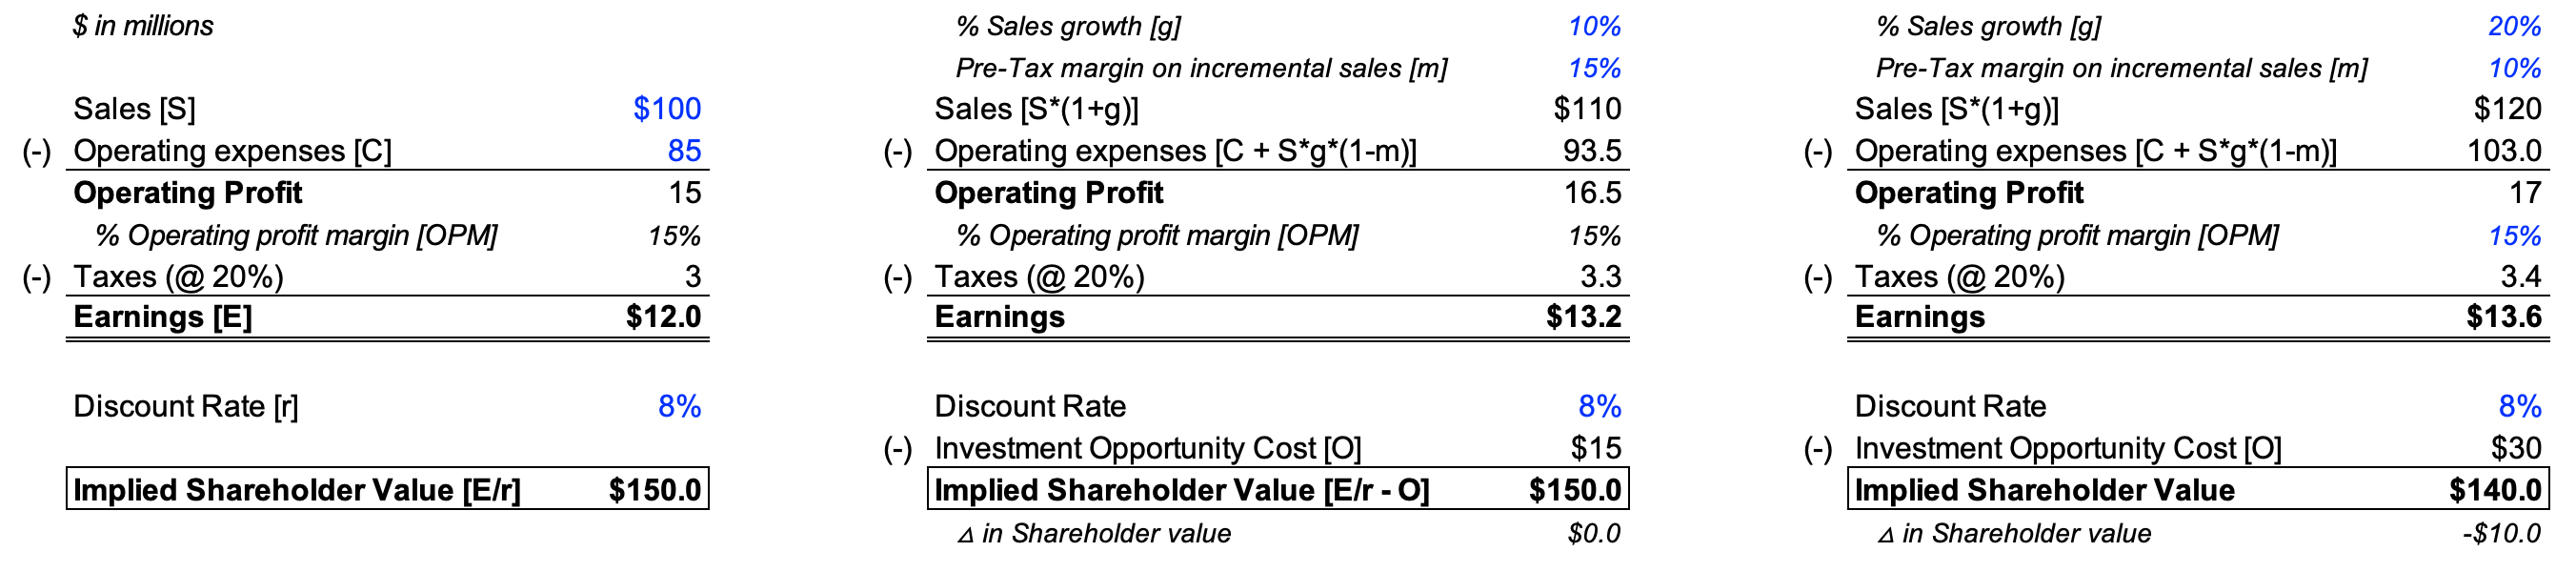
\includegraphics[scale=0.33]{/Users/rishiratan/OneDrive/Learning/Hedge Funds Investing/Investing-Book-Reviews/imgs/EPS_Fallacy.png}
\label{fig:parametric}
\end{figure}
\section{Chapter 2: How the Market Values Stocks}
\textbf{Compounding}: dollar today is worth more than dollar in the future because you can invest today's dollar and earn a positive rate of return. 
\vspace {0.3 cm}
  \newline
\textbf{Discounting}: future cash flow is converted into its equivalent present value. Discounting is the opposite of compounding. 
\vspace {0.3 cm}
  \newline
\textbf{Present Value}: an asset's present value = sum of its expected cash flows discounted by an expected rate of return. Maximum price an investor should pay for an asset. 
\vspace {0.3 cm}
  \newline
\textbf{Return}: what investors anticipate earning on assets with similar risk. 
\vspace {0.3 cm}
  \newline
\textbf{Bond Prices}: present value of the contractual cash flows discounted at the current expected rare of return. The market sets prices so that expected returns match the perceived risk. 
\begin{tcolorbox}[colback=blue!5!white,colframe=blue!75!black]
    Whereas bonds contractually specify cash flows and date when principal is to be repaid, stocks have uncertain cash flows, an indefinite life, and no provision for repayment. That greater uncertainty makes stocks more difficult to value than bonds. 
    \vspace {0.3 cm}
      \newline
    Purpose of any stock market, is simply to provide liquidity for stocks in return for the promise of future cash flows, enabling investors to realize the present value of a future stream of income at any time.
    \begin{itemize}
        \item Market prices respond to changes in a company's prospectus for cash flow. 
        \item Market prices reflect cash flows well into the future. 
        \item Companies often need 10-20 years(for more competitive industries) of value creating cash flows to justify their stock price
    \end{itemize}
    Static measures of near-term (3-5 years) don't capture future performance and ultimately let investors down, especially in a global economy marked by spirited compeition and disruptive technologies. An investor cannot convincingly conclude that a stock is undervalues or overvalued without assessing a company's future cash flows.
\end{tcolorbox}
\begin{figure}[H]
    \centering
    
\includegraphics[scale = 0.65]{/Users/rishiratan/OneDrive/Learning/Hedge Funds Investing/Investing-Book-Reviews/imgs/Shareholder_ValueMap.png}
\end{figure}

\begin{itemize}
    \item Sales growth [g] and operating profit margin [OPM] determine operating profit
    \item NOPAT = Operating profit (-) Cash Taxes
    \item FCF = NOPAT - investments in WC and fixed assets. Thus, free cash flow is the pool of cash available to pay the claims of debtholders and shareholders. 
    \item Shareholder Value = Corporate Value + Non Operating Assets (-) Market Value of Debt and other relevant liabilities
\end{itemize}

\begin{tcolorbox}[colback=blue!5!white,colframe=blue!75!black]
Expectations investing reverses the above descibed standard DCF model by starting with price, which may differ from value, and determines the expectations for cash flows that the price implies. 
\vspace {0.3 cm}
  \newline
Three operating value drivers: 
\begin{itemize}
    \item sales growth [g]
    \item operating profit margin [OPM]
    \item incremental investment rate [i]
\end{itemize}
Value determinant: cash tax rate [T]
\end{tcolorbox}
\begin{figure}[H]
    \centering
    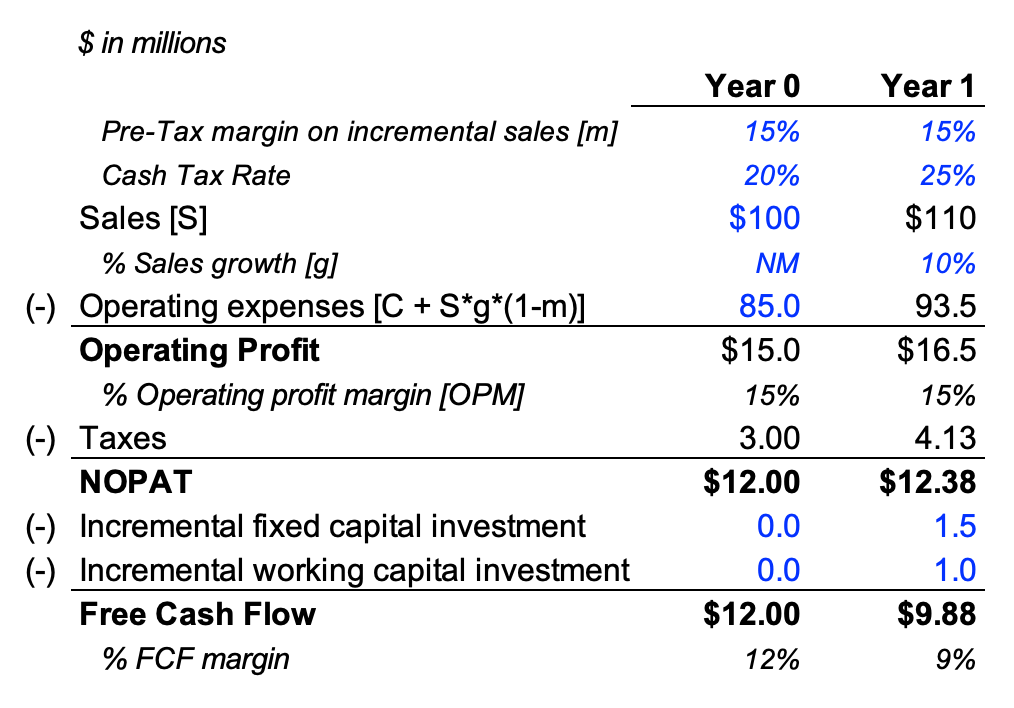
\includegraphics[scale = 0.55]{/Users/rishiratan/OneDrive/Learning/Hedge Funds Investing/Investing-Book-Reviews/imgs/FCF.png}
\end{figure}

Because we want to calculate FCF, we exclude the amortization of acquired intangible assets, which is a non-cash expense. 
Embedded interest in lease expense is also excluded since that is considered a financing cost
Depreciation expense remains as part of the OPM even though its a noncash item. But it is deducted from the CapEx so that the FCF is truly a cash figure. 
Tax expense in the income statement, book taxes, is often greater than the actual payments, or cash taxes, during a given period. This is because companies can recognize some revenue and expense items at different times for book versus tax purposes. 
Company might use an accelerated depreciation for tax purposes such that the result is higher than straight-line depreciation, thereby, increasing the company's expenses and reducing its cash tax bill. This results in a deferred tax asset.
Stock based compensation (SBC) can also create timing differences between cash and reported taxes. As a result, cash tax rates are commonly lower than book tax rates. 
Cash tax rate represents taxes payable on operating profit, not on pre-tax income. Therefore, to calculate the taxes that a company would pay if it were entirely equity financed, we must remove the tax effects of interest expense and non-operating income or expenses. 
Removing the tax benefit of interest expense deductions, interest expense x tax rate, increases the cash tax bill, and removing the taxes on operating profit. 
Fixed capital investment includes CapEx and Depreciation expense. Rate of fixed capital investment required for the company to sustain its operations is calculated as a \% of sales increase. i.e. (CapEx - Depreciation) / change in sales. 
As a business operating working capital generally grows proportionally. 
Inventories generally rise as sales increase and rising inventory requires cash payments for materials, labor, and overhead. Since COGS excludes cash outlays it has to be included in working capital calculation. 

\begin{tcolorbox}[colback=blue!5!white,colframe=blue!75!black]
Amazon is an unique company in that working capital is actually a source of cash instead of an outlay since the company receives cash from customers before it has to pay its suppliers. 
\vspace {0.3 cm}
  \newline
FCFs only represent a tiny fraction of the company's value as most of the value relies in residual value aka terminal value. 
\end{tcolorbox}

Four ways to estimate terminal value: 
perpetuity growth: 
perpetuity growth with inflation:
perpetuity growth with partial inflation:
perpetuity with decline:

Value factors: 
\begin{itemize}
    \item  volume
    \item rice and mix
    \item operating leverage
    \item economies of scale
    \item cost efficiencies
    \item investment efficiencies
\end{itemize}

\end{document}